\documentclass[9pt,a4paper,]{extarticle}

\usepackage{f1000_styles}

\usepackage[pdfborder={0 0 0}]{hyperref}

\usepackage[numbers]{natbib}
\bibliographystyle{unsrtnat}


%% maxwidth is the original width if it is less than linewidth
%% otherwise use linewidth (to make sure the graphics do not exceed the margin)
\makeatletter
\def\maxwidth{ %
  \ifdim\Gin@nat@width>\linewidth
    \linewidth
  \else
    \Gin@nat@width
  \fi
}
\makeatother

\usepackage{color}
\usepackage{fancyvrb}
\newcommand{\VerbBar}{|}
\newcommand{\VERB}{\Verb[commandchars=\\\{\}]}
\DefineVerbatimEnvironment{Highlighting}{Verbatim}{commandchars=\\\{\}}
% Add ',fontsize=\small' for more characters per line
\usepackage{framed}
\definecolor{shadecolor}{RGB}{248,248,248}
\newenvironment{Shaded}{\begin{snugshade}}{\end{snugshade}}
\newcommand{\AlertTok}[1]{\textcolor[rgb]{0.94,0.16,0.16}{#1}}
\newcommand{\AnnotationTok}[1]{\textcolor[rgb]{0.56,0.35,0.01}{\textbf{\textit{#1}}}}
\newcommand{\AttributeTok}[1]{\textcolor[rgb]{0.77,0.63,0.00}{#1}}
\newcommand{\BaseNTok}[1]{\textcolor[rgb]{0.00,0.00,0.81}{#1}}
\newcommand{\BuiltInTok}[1]{#1}
\newcommand{\CharTok}[1]{\textcolor[rgb]{0.31,0.60,0.02}{#1}}
\newcommand{\CommentTok}[1]{\textcolor[rgb]{0.56,0.35,0.01}{\textit{#1}}}
\newcommand{\CommentVarTok}[1]{\textcolor[rgb]{0.56,0.35,0.01}{\textbf{\textit{#1}}}}
\newcommand{\ConstantTok}[1]{\textcolor[rgb]{0.00,0.00,0.00}{#1}}
\newcommand{\ControlFlowTok}[1]{\textcolor[rgb]{0.13,0.29,0.53}{\textbf{#1}}}
\newcommand{\DataTypeTok}[1]{\textcolor[rgb]{0.13,0.29,0.53}{#1}}
\newcommand{\DecValTok}[1]{\textcolor[rgb]{0.00,0.00,0.81}{#1}}
\newcommand{\DocumentationTok}[1]{\textcolor[rgb]{0.56,0.35,0.01}{\textbf{\textit{#1}}}}
\newcommand{\ErrorTok}[1]{\textcolor[rgb]{0.64,0.00,0.00}{\textbf{#1}}}
\newcommand{\ExtensionTok}[1]{#1}
\newcommand{\FloatTok}[1]{\textcolor[rgb]{0.00,0.00,0.81}{#1}}
\newcommand{\FunctionTok}[1]{\textcolor[rgb]{0.00,0.00,0.00}{#1}}
\newcommand{\ImportTok}[1]{#1}
\newcommand{\InformationTok}[1]{\textcolor[rgb]{0.56,0.35,0.01}{\textbf{\textit{#1}}}}
\newcommand{\KeywordTok}[1]{\textcolor[rgb]{0.13,0.29,0.53}{\textbf{#1}}}
\newcommand{\NormalTok}[1]{#1}
\newcommand{\OperatorTok}[1]{\textcolor[rgb]{0.81,0.36,0.00}{\textbf{#1}}}
\newcommand{\OtherTok}[1]{\textcolor[rgb]{0.56,0.35,0.01}{#1}}
\newcommand{\PreprocessorTok}[1]{\textcolor[rgb]{0.56,0.35,0.01}{\textit{#1}}}
\newcommand{\RegionMarkerTok}[1]{#1}
\newcommand{\SpecialCharTok}[1]{\textcolor[rgb]{0.00,0.00,0.00}{#1}}
\newcommand{\SpecialStringTok}[1]{\textcolor[rgb]{0.31,0.60,0.02}{#1}}
\newcommand{\StringTok}[1]{\textcolor[rgb]{0.31,0.60,0.02}{#1}}
\newcommand{\VariableTok}[1]{\textcolor[rgb]{0.00,0.00,0.00}{#1}}
\newcommand{\VerbatimStringTok}[1]{\textcolor[rgb]{0.31,0.60,0.02}{#1}}
\newcommand{\WarningTok}[1]{\textcolor[rgb]{0.56,0.35,0.01}{\textbf{\textit{#1}}}}

% disable code chunks background
%\renewenvironment{Shaded}{}{}

% disable section numbers
\setcounter{secnumdepth}{0}

%% added by MLS, this is not in the F1000 style by default %%

\hypersetup{unicode=true,
            pdftitle={BASiCS workflow: a step-by-step analysis of expression variability using single cell RNA sequencing data},
            pdfkeywords={Single-cell RNA sequencing, expression variability, transcriptional noise, differential expression testing},
            colorlinks=true,
            linkcolor=Maroon,
            citecolor=Blue,
            urlcolor=Orange,
            breaklinks=true}

%% End added by MLS %%

\setlength{\parindent}{0pt}
\setlength{\parskip}{6pt plus 2pt minus 1pt}



\begin{document}
\pagestyle{front}

\title{BASiCS workflow: a step-by-step analysis of expression variability using single cell RNA sequencing data}

\author[1,2,3]{Nils Eling}
\author[4]{Alan O'Callaghan\thanks{\ttfamily a.b.o'callaghan@sms.ed.ac.uk}}
\author[1,2]{John C. Marioni}
\author[4,5]{Catalina A. Vallejos\thanks{\ttfamily catalina.vallejos@igmm.ed.ac.uk}}
\affil[1]{European Molecular Biology Laboratory, European Bioinformatics Institute, Wellcome Trust Genome Campus, Hinxton, Cambridge CB10 1SD, UK}
\affil[2]{Cancer Research UK Cambridge Institute, University of Cambridge, Li Ka Shing Centre, Cambridge, CB2 0RE, UK}
\affil[3]{Department of Quantitative Biomedicine, University of Zurich, Winterthurerstrasse 190, CH-8057, Zurich, Switzerland}
\affil[4]{MRC Human Genetics Unit, Institute of Genetics \& Molecular Medicine, University of Edinburgh, Western General Hospital, Crewe Road, Edinburgh, EH4 2XU, UK}
\affil[5]{The Alan Turing Institute, British Library, 96 Euston Road, London, NW1 2DB, UK}

\maketitle
\thispagestyle{front}

\begin{abstract}
Cell-to-cell gene expression variability is an inherent feature of complex
biological systems, such as immunity and development. Single-cell RNA
sequencing is a powerful tool to quantify this heterogeneity, but it is prone
to strong technical noise. In this article, we describe a step-by-step
computational workflow which uses the BASiCS Bioconductor package to robustly
quantify expression variability within and between known groups of cells (such
as experimental conditions or cell types). BASiCS uses an integrated framework
for data normalisation, technical noise quantification and downstream
analyses, whilst propagating statistical uncertainty across these steps.
Within a single seemingly homogeneous cell population, BASiCS can identify
highly variable genes that exhibit strong heterogeneity as well as lowly
variable genes with stable expression. BASiCS also uses a probabilistic
decision rule to identify changes in expression variability between cell
populations, whilst avoiding confounding effects related to differences in
technical noise or in overall abundance. Using two publicly available
datasets, we guide users through a complete pipeline which includes
preliminary steps for quality control as well as data exploration
using the scater and scran Bioconductor packages. Data for the first case
study was generated using the Fluidigm@ C1 system, in which extrinsic
spike-in RNA molecules were added as a control. The second dataset was
generated using a droplet-based system, for which spike-in RNA is not
available. This analysis provides an example, in which differential
variability testing reveals insights regarding a possible early cell fate
commitment process. The workflow is accompanied by a Docker image that
ensures the reproducibility of our results.
\end{abstract}

\section*{Keywords}
Single-cell RNA sequencing, expression variability, transcriptional noise, differential expression testing


\clearpage
\pagestyle{main}

\hypertarget{introduction}{%
\section{Introduction}\label{introduction}}

Single-cell RNA-sequencing (scRNA-seq) enables the study of genome-wide
transcriptional heterogeneity in cell populations that cannot be
detected in bulk experiments \citep{Stegle2015, Prakadan2017, Patange2018}.
On the broadest level, this heterogeneity can reflect the presence of distinct
cell subtypes or states.
Alternatively, it can be due to gradual changes along biological processes, such
as development and differentiation.
Several clustering and pseudotime inference methods have been developed to
characterise these types of heterogeneity \citep{Kiselev2019, Saelens2019}.
However, there is a limited availability of computational tools tailored
to study more subtle variability within seemingly homogeneous cell populations.
This variability can reflect deterministic or stochastic events that regulate
gene expression and, among others, has been reported to increase prior to cell
fate decisions \citep{Mojtahedi2016} as well as during ageing \citep{Martinez-jimenez2017}.

This article complements existing scRNA-seq workflows based on the
Bioconductor package ecosystem (e.g. \citep{Lun2016, Kim2019}).
We describe a step-by-step analysis which uses \emph{\href{https://bioconductor.org/packages/3.11/scater}{scater}} and
\emph{\href{https://bioconductor.org/packages/3.11/scran}{scran}} to perform quality control (QC) as well as
initial exploratory analyses \citep{McCarthy2017, Lun2016}.
To robustly quantify transcriptional variability we use \emph{\href{https://bioconductor.org/packages/3.11/BASiCS}{BASiCS}} \citep{Vallejos2015, Vallejos2016, Eling2017} --- a Bayesian hierarchical framework
that jointly performs data normalisation (global scaling), technical noise
quantification and downstream analyses, whilst propagating statistical
uncertainty across these steps.
Among others, \emph{\href{https://bioconductor.org/packages/3.11/BASiCS}{BASiCS}}, has led to new insights about the
heterogeneity of immune cells \citep{Martinez-jimenez2017}.

Within a population of cells, \emph{\href{https://bioconductor.org/packages/3.11/BASiCS}{BASiCS}} decomposes the total
observed variability in expression measurements into technical and biological
components \citep{Vallejos2015}.
This enables the identification of \emph{highly variable genes} (HVGs) that capture
the major sources of heterogeneity within the analysed cells \citep{Brennecke2013}.
HVG detection is often used as feature selection, to identify the input
set of genes for subsequent analyses.
\emph{\href{https://bioconductor.org/packages/3.11/BASiCS}{BASiCS}} can also highlight \emph{lowly variable genes} (LVGs) that
exhibit stable expression across the population of cells.
These may relate to essential cellular functions and can assist the development
of new data normalisation or integration strategies \citep{Lin2019}.

\emph{\href{https://bioconductor.org/packages/3.11/BASiCS}{BASiCS}} also provides a probabilistic decision rule to
perform differential expression analyses between two (or more) pre-specified
groups of cells \citep{Vallejos2016, Eling2018}.
Whilst several differential expression tools have been proposed for scRNA-seq
data (e.g. \citep{Kharchenko2014, Finak2015}), some evidence suggests that
these do not generally outperform popular bulk RNA-seq tools \citep{Soneson2018}.
Moreover, most of these methods are only designed to uncover changes in overall
expression, ignoring the more complex patterns that can arise at the single cell
level \citep{Lahnemann2020}.
Instead, \emph{\href{https://bioconductor.org/packages/3.11/BASiCS}{BASiCS}} embraces the high granularity of scRNA-seq data,
uncovering changes in cell-to-cell expression variability that are not
confounded by differences in technical noise or in overall expression.

Here, we briefly discuss the sources of variability that arise in scRNA-seq data
and some of the strategies that have been designed to control or attenuate
technical noise in these assays.
We also summarise the main features of the Bioconductor packages used
throughout this workflow, and provide a description for the underlying
statistical model implemented in \emph{\href{https://bioconductor.org/packages/3.11/BASiCS}{BASiCS}}.
This includes practical guidance to assess the convergence of the Markov Chain
Monte Carlo (MCMC) algorithm that is used to infer model parameters as well as
recommendations to interpret and post-process the model outputs.
Finally, we provide a step-by-step case study.

All source code used to generate the results presented in this article is
available \href{https://github.com/VallejosGroup/BASiCSWorkflow}{on Github}.
To ensure the
reproducibility of this workflow, the analysis environment and all software
dependencies are provided as a Docker image \citep{Boettiger2015}. The image
can be obtained from
\href{https://hub.docker.com/repository/docker/alanocallaghan/bocker}{Docker Hub}.

\hypertarget{sources-of-variability-in-scrna-seq-data}{%
\section{Sources of variability in scRNA-seq data}\label{sources-of-variability-in-scrna-seq-data}}

The focus of this article is to quantify the magnitude of cell-to-cell
expression heterogeneity within seemingly homogeneous cell populations.
Here, we briefly describe the underlying sources of heterogeneity that can be
captured by cell-to-cell variability estimates derived from scRNA-seq data.

Stochastic variability within a cell population --- often referred to as
transcriptional \emph{noise} --- can arise from intrinsic and extrinsic sources
\citep{Elowitz2002, Eling2019}.
Classically, extrinsic noise is defined as stochastic fluctuations induced by
different dynamic cellular states (e.g.~cell cycle, metabolism, intra- and
inter-cellular signalling)
\citep{Zopf2013, Iwamoto2016, Kiviet2014}.
In contrast, intrinsic noise arises from stochastic effects on biochemical
processes such as transcription and translation \citep{Elowitz2002}.
Intrinsic noise can be modulated by genetic and epigenetic modifications (such
as mutations, histone modifications, CpG island length and nucleosome
positioning) \citep{Eberwine2015, Faure2017, Morgan2018} and is usually measured
at the gene level \citep{Elowitz2002}.
Cell-to-cell gene expression variability estimates derived from scRNA-seq data
capture a combination of these effects, as well as deterministic regulatory
mechanisms \citep{Eling2019}.
Moreover, these variability estimates can also be inflated by the technical
noise that is typically observed in scRNA-seq data \citep{Brennecke2013}.

Different strategies have been incorporated into scRNA-seq protocols to control
or attenuate technical noise.
For example, external RNA spike-in molecules (such as the set introduced by the
External RNA Controls Consortium, ERCC \citep{Rna2005}) can be added to each cell's
lysate in a (theoretically) known fixed quantity.
Spike-ins can assist quality control steps \citep{McCarthy2017}, data normalisation
\citep{Vallejos2017} and can be used to infer technical noise \citep{Brennecke2013}.
Another strategy is to tag individual cDNA molecules using unique molecular
identifiers (UMIs) before PCR amplification \citep{Islam2014}.
Reads that contain the same UMI can be collapsed into a single molecule count,
attenuating technical variability associated to cell-to-cell differences
in amplification and sequencing depth (these technical biases are not fully
removed unless sequencing to saturation \citep{Vallejos2017}).
However, despite the benefits associated to the use of spike-ins and UMIs,
these are not available for all scRNA-seq protocols \citep{Haque2017}.

\hypertarget{methods}{%
\section{Methods}\label{methods}}

This step-by-step scRNA-seq workflow is primarily based on the Bioconductor
package ecosystem \citep{Amezquita2019}.
A graphical overview is provided in Figure \ref{fig:overview}
and its main components are described below.

\begin{figure}

{\centering 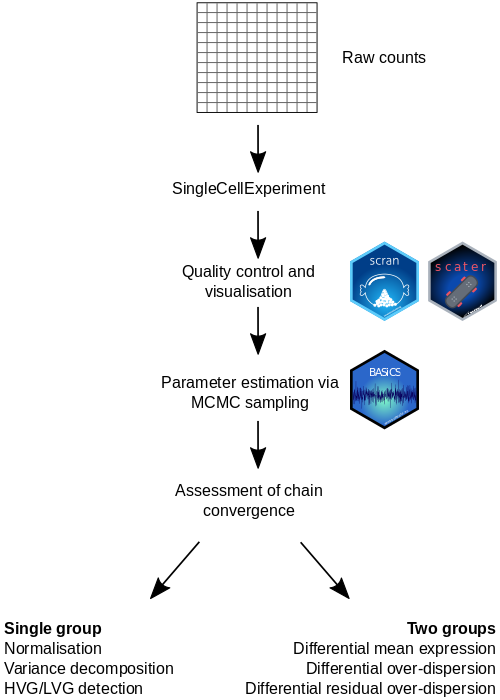
\includegraphics[width=2.5in,height=3.5in]{figure/Overview} 

}

\caption{Graphical overview for the scRNA-seq analysis workflow described in this manuscript. Starting from a matrix of expression counts, we use the scater and scran Bioconductor packages to perform QC and initial exploratory analyses. To robustly quantify transcriptional heterogeneity within seemingly homogeneous cell populations, we apply the BASiCS Bioconductor package and  illustrate how BASiCS can be used to analyse a single or multiple pre-specified groups of cells.}\label{fig:overview}
\end{figure}

\hypertarget{input-data}{%
\subsection{Input data}\label{input-data}}

\begin{Shaded}
\begin{Highlighting}[]
\KeywordTok{library}\NormalTok{(}\StringTok{"SingleCellExperiment"}\NormalTok{)}
\end{Highlighting}
\end{Shaded}

We use \emph{\href{https://bioconductor.org/packages/3.11/SingleCellExperiment}{SingleCellExperiment}} to convert an input
matrix of raw read-counts (molecule counts for UMI-based protocols) into a
\texttt{SingleCellExperiment} object which can also store its associated
metadata, such as gene- and cell-specific information.
Moreover, when available, the same object can also store read-counts for
spike-in molecules (see \texttt{altExp()}).
A major advantage of using a \texttt{SingleCellExperiment} object as the input for
scRNA-seq analyses is the interoperability across a large number of
Bioconductor packages \citep{Amezquita2019}.

\hypertarget{quality-control-and-exploratory-analysis}{%
\subsection{Quality control and exploratory analysis}\label{quality-control-and-exploratory-analysis}}

\begin{Shaded}
\begin{Highlighting}[]
\KeywordTok{library}\NormalTok{(}\StringTok{"scater"}\NormalTok{)}
\KeywordTok{library}\NormalTok{(}\StringTok{"scran"}\NormalTok{)}
\KeywordTok{library}\NormalTok{(}\StringTok{"ggplot2"}\NormalTok{)}
\end{Highlighting}
\end{Shaded}

An critical step in scRNA-seq analyses is to apply QC diagnostics, removing low
quality samples that may distort downstream analyses.
Among others, QC can help to identify samples that contain broken cells, that
are empty or that contain multiple cells \citep{Ilicic2016}.
Moreover, lowly expressed genes for which less reliable information is
available are typically also removed.
The \href{https://osca.bioconductor.org/}{\emph{OSCA}} online book provides an extensive
overview on important aspects of how to perform QC of scRNA-seq data, including
exploratory analyses \citep{Amezquita2019}.

To perform QC, we use the \emph{\href{https://bioconductor.org/packages/3.11/scater}{scater}} package \citep{McCarthy2017}.
The \texttt{addPerCellQC} and \texttt{addPerFeatureQC} functions are applied to calculate
QC metrics for each cell (e.g.~total read-count) and gene (e.g.~percentage of
zeroes across all cells), respectively.
The package also provides a suite of visualisation tools that can be used to
explore the data under study and its associated QC diagnostic metrics.

The \emph{\href{https://bioconductor.org/packages/3.11/scran}{scran}} package offers additional tools for QC
diagnostics and a variety of functions scRNA-seq data analysis \citep{Lun2016}.
It can perform \emph{global scaling} normalisation, calculating cell-specific
scaling factors that capture global differences in read-counts across cells
(e.g.~due to sequencing depth and PCR amplification) \citep{Lun2016pooling}.
To explore the strenght of transcriptional variability, we use the \texttt{modelGeneCV2}
function to infer an overall trend between mean expression and the
squared coefficent of variation (CV\textsuperscript{2}) for each gene.
To derive gene-specific variability estimates that are not confounded by this
overall trend, the \texttt{DM} function calculates the distance between CV\(^2\) and a
rolling median along the range of mean expression values \citep{Kolodziejczyk2015cell}.
DM estimates enable exploratory analyses of cell-to-cell heterogeneity, but a
measure of uncertainty is not readily available. As such, gene-specific
downstream inference (e.g.~differential variability testing) is precluded.

Finally, we also load \emph{\href{https://CRAN.R-project.org/package=ggplot2}{ggplot2}} to visualise the results of these
analyses.

\hypertarget{analysis-of-cell-to-cell-transcriptional-variability}{%
\subsection{Analysis of cell-to-cell transcriptional variability}\label{analysis-of-cell-to-cell-transcriptional-variability}}

\begin{Shaded}
\begin{Highlighting}[]
\KeywordTok{library}\NormalTok{(}\StringTok{"BASiCS"}\NormalTok{)}
\end{Highlighting}
\end{Shaded}

The \emph{\href{https://bioconductor.org/packages/3.11/BASiCS}{BASiCS}} package uses a Bayesian hierarchical framework
that borrows information across all genes and cells to robustly quantify
transcriptional variability \citep{Vallejos2015BASiCS}.
Similar to the approach adopted in \emph{\href{https://bioconductor.org/packages/3.11/scran}{scran}}, \emph{\href{https://bioconductor.org/packages/3.11/BASiCS}{BASiCS}}
infers cell-specific global scaling normalisation parameters.
However, instead of inferring these as a pre-processing step,
\emph{\href{https://bioconductor.org/packages/3.11/BASiCS}{BASiCS}} uses an integrated approach in which data normalisation
and downstream analyses are performed simultaneously, thereby propagating
statistical uncertainty.
To quantify technical noise, the original implementation of
\emph{\href{https://bioconductor.org/packages/3.11/BASiCS}{BASiCS}} uses information from extrinsic spike-in molecules as
control features, but the model has been extended to address situations in which
spike-ins are not available \citep{Eling2018}.

\emph{\href{https://bioconductor.org/packages/3.11/BASiCS}{BASiCS}} summarises expression patterns through
gene-specific \emph{mean} (\(\mu_i\)) and \emph{over-dispersion} (\(\delta_i\)) parameters.
Mean parameters \(\mu_i\) quantify the overall expression for each gene \(i\)
across the population of cells under study.
In contrast, \(\delta_i\) captures the excess of variability that is observed with
respect to what would be expected in a homogeneous cell population, after
taking into account technical noise.
This is used as a proxy to quantify transcriptional variability.
Moreover, to account for the strong association that is typically observed
between mean expression and over-dispersion estimates, we recently introduced
gene-specific \emph{residual over-dispersion} parameters \(\epsilon_i\) \citep{Eling2018}.
Similar to DM values implemented in \emph{\href{https://bioconductor.org/packages/3.11/scran}{scran}}, these are defined as
deviations with respect to an overall regression trend that captures the
relationship between mean and over-dispersion values.

Parameter inference is implemented in the \texttt{BASiCS\_MCMC} function using an
adaptive Metropolis within Gibbs algorithm \citep{Roberts2009}, whose convergence can
be assessed using the \texttt{BASiCS\_DiagHist} and \texttt{BASiCS\_DiagPlot} functions,
among others.

The output from \texttt{BASiCS\_MCMC} is a \texttt{BASiCS\_Chain} object, which can be used
for further downstream analyses. In particular, \texttt{BASiCS\_DetectHVG} and
\texttt{BASiCS\_DetectLVG} can be respectively used to identify highly and lowly
variable genes within a cell population. Moreover, \texttt{BASiCS\_TestDE} is used to
perform differential mean and variability analyses between groups of cells.

\hypertarget{Tcells}{%
\section{\texorpdfstring{Case study: analysis of naive CD4\textsuperscript{+} T cells}{Case study: analysis of naive CD4+ T cells}}\label{Tcells}}

As a case study, we use scRNA-seq data generated for CD4\textsuperscript{+} T cells
using the C1 Single-Cell Auto Prep System (Fluidigm\textsuperscript{®}).
Martinez-Jimenez \emph{et al.} profiled naive (hereafter also referred to as
\emph{unstimulated}) and activated (3 hours using \emph{in vitro} antibody stimulation)
CD4\textsuperscript{+} T cells from young and old animals across two mouse strains to study
changes in expression variability during ageing and upon immune activation
\citep{Martinez-jimenez2017}.
They extracted naive or effector memory CD4\textsuperscript{+} T cells from spleens of young or
old animals, obtaining purified populations using either magnetic-activated cell
sorting (MACS) or fluorescence activated cell sorting (FACS).
External ERCC spike-in RNA \citep{Rna2005} was added to aid the quantification of
technical variability across all cells and all experiments were performed in
replicates (also referred to as batches) to control for batch effects.

\hypertarget{obtaining-the-data}{%
\subsection{Obtaining the data}\label{obtaining-the-data}}

The matrix with raw read counts can be obtained from ArrayExpress under the
accession number
\href{https://www.ebi.ac.uk/arrayexpress/experiments/E-MTAB-4888/}{E-MTAB-4888}.
In the matrix, column names contain library identifiers and row names
display gene Ensembl identifiers.

\begin{Shaded}
\begin{Highlighting}[]
\ControlFlowTok{if}\NormalTok{ (}\OperatorTok{!}\KeywordTok{file.exists}\NormalTok{(}\StringTok{"downloads/raw_data.txt"}\NormalTok{)) \{}
  \CommentTok{# Download raw counts file}
\NormalTok{  website <-}\StringTok{ "https://www.ebi.ac.uk/"}
\NormalTok{  folder <-}\StringTok{ "arrayexpress/files/E-MTAB-4888/"}
\NormalTok{  file <-}\StringTok{ "E-MTAB-4888.processed.1.zip"}
\NormalTok{  destfile <-}\StringTok{ "downloads/raw_data.txt.zip"}
  \KeywordTok{download.file}\NormalTok{(}
    \KeywordTok{paste0}\NormalTok{(website, folder, file),}
    \DataTypeTok{destfile =}\NormalTok{ destfile}
\NormalTok{  )}
  \KeywordTok{unzip}\NormalTok{(}\StringTok{"downloads/raw_data.txt.zip"}\NormalTok{, }\DataTypeTok{exdir =} \StringTok{"downloads"}\NormalTok{)}
  \KeywordTok{file.remove}\NormalTok{(}\StringTok{"downloads/raw_data.txt.zip"}\NormalTok{)}
\NormalTok{\}}

\CommentTok{# Read in raw data}
\NormalTok{CD4_raw <-}\StringTok{ }\KeywordTok{read.table}\NormalTok{(}\StringTok{"downloads/raw_data.txt"}\NormalTok{, }\DataTypeTok{header =} \OtherTok{TRUE}\NormalTok{, }\DataTypeTok{sep =} \StringTok{"}\CharTok{\textbackslash{}t}\StringTok{"}\NormalTok{)}
\NormalTok{CD4_raw <-}\StringTok{ }\KeywordTok{as.matrix}\NormalTok{(CD4_raw)}
\end{Highlighting}
\end{Shaded}

The input matrix contains data for 1,513
cells and 31,181
genes (including 92 ERCC spike-ins).
Information about experimental conditions and batches is available in a metadata
file under the same accession number.

\begin{Shaded}
\begin{Highlighting}[]
\ControlFlowTok{if}\NormalTok{ (}\OperatorTok{!}\KeywordTok{file.exists}\NormalTok{(}\StringTok{"downloads/metadata_file.txt"}\NormalTok{)) \{}
  \CommentTok{# Download raw counts file}
\NormalTok{  website <-}\StringTok{ "https://www.ebi.ac.uk/"}
\NormalTok{  folder <-}\StringTok{ "arrayexpress/files/E-MTAB-4888/"}
\NormalTok{  file <-}\StringTok{ "E-MTAB-4888.additional.1.zip"}
\NormalTok{  destfile <-}\StringTok{ "downloads/metadata.txt.zip"}
  \KeywordTok{download.file}\NormalTok{(}
    \KeywordTok{paste0}\NormalTok{(website, folder, file),}
    \DataTypeTok{destfile =}\NormalTok{ destfile}
\NormalTok{  )}
  \KeywordTok{unzip}\NormalTok{(}\StringTok{"downloads/metadata.txt.zip"}\NormalTok{, }\DataTypeTok{exdir =} \StringTok{"downloads"}\NormalTok{)}
  \KeywordTok{file.remove}\NormalTok{(}\StringTok{"downloads/metadata.txt.zip"}\NormalTok{)}
\NormalTok{\}}
\CommentTok{# Read in metadata file}
\NormalTok{CD4_metadata <-}\StringTok{ }\KeywordTok{read.table}\NormalTok{(}
  \StringTok{"downloads/metadata_file.txt"}\NormalTok{,}
  \DataTypeTok{header =} \OtherTok{TRUE}\NormalTok{,}
  \DataTypeTok{sep =} \StringTok{"}\CharTok{\textbackslash{}t}\StringTok{"}
\NormalTok{)}

\CommentTok{# Save library identifier as rownames}
\KeywordTok{rownames}\NormalTok{(CD4_metadata) <-}\StringTok{ }\NormalTok{CD4_metadata}\OperatorTok{$}\NormalTok{X}

\CommentTok{# Show metadata entries}
\KeywordTok{names}\NormalTok{(CD4_metadata)}
\end{Highlighting}
\end{Shaded}

\begin{verbatim}
## [1] "X"           "Strain"      "Age"         "Stimulus"    "Individuals"
## [6] "Celltype"
\end{verbatim}

The metadata contains library identifiers (\texttt{X}), strain information (\texttt{Strain};
\emph{Mus musculus castaneus} or \emph{Mus musculus domesticus}), the age of the animals
(\texttt{Age}; young or old), stimulation state of the cells (\texttt{Stimulus}; naive or
activated), batch information (\texttt{Individuals}; associated to different mice),
and cell type information (\texttt{Celltype}; via FACS or MACS purification).

The data and metadata described above are then converted into a
\emph{\href{https://bioconductor.org/packages/3.11/SingleCellExperiment}{SingleCellExperiment}} object.

\begin{Shaded}
\begin{Highlighting}[]
\CommentTok{# Separate intrinsic from ERCC counts}
\NormalTok{bio_counts <-}\StringTok{ }\NormalTok{CD4_raw[}\OperatorTok{!}\KeywordTok{grepl}\NormalTok{(}\StringTok{"ERCC"}\NormalTok{, }\KeywordTok{rownames}\NormalTok{(CD4_raw)), ]}
\NormalTok{spike_counts <-}\StringTok{ }\NormalTok{CD4_raw[}\KeywordTok{grepl}\NormalTok{(}\StringTok{"ERCC"}\NormalTok{, }\KeywordTok{rownames}\NormalTok{(CD4_raw)), ]}
\CommentTok{# Generate the SingleCellExperiment object}
\NormalTok{sce_CD4_all <-}\StringTok{ }\KeywordTok{SingleCellExperiment}\NormalTok{(}
  \DataTypeTok{assays =} \KeywordTok{list}\NormalTok{(}\DataTypeTok{counts =} \KeywordTok{as.matrix}\NormalTok{(bio_counts)),}
  \DataTypeTok{colData =}\NormalTok{ CD4_metadata[}\KeywordTok{colnames}\NormalTok{(CD4_raw), ]}
\NormalTok{)}
\CommentTok{# Add read-counts for spike-ins }
\KeywordTok{altExp}\NormalTok{(sce_CD4_all, }\StringTok{"spike-ins"}\NormalTok{) <-}\StringTok{ }\KeywordTok{SummarizedExperiment}\NormalTok{(}
  \DataTypeTok{assays =} \KeywordTok{list}\NormalTok{(}\DataTypeTok{counts =}\NormalTok{ spike_counts)}
\NormalTok{)}
\NormalTok{sce_CD4_all}
\end{Highlighting}
\end{Shaded}

\begin{verbatim}
## class: SingleCellExperiment 
## dim: 31089 1513 
## metadata(0):
## assays(1): counts
## rownames(31089): ENSMUSG00000000001 ENSMUSG00000000003 ...
##   ENSMUSG00000106668 ENSMUSG00000106670
## rowData names(0):
## colnames(1513): do4737 do4739 ... do12254 do12257
## colData names(6): X Strain ... Individuals Celltype
## reducedDimNames(0):
## altExpNames(1): spike-ins
\end{verbatim}

Throughout our analysis, we focus on naive and activated CD4\textsuperscript{+} T cells obtained
from young \emph{Mus musculus domesticus} animals, purified using MACS-based cell sorting.
The following code is used to extract these
146 samples from the full dataset.

\begin{Shaded}
\begin{Highlighting}[]
\NormalTok{ind_select <-}\StringTok{ }\NormalTok{sce_CD4_all}\OperatorTok{$}\NormalTok{Strain }\OperatorTok{==}\StringTok{ "Mus musculus domesticus"} \OperatorTok{&}
\StringTok{  }\NormalTok{sce_CD4_all}\OperatorTok{$}\NormalTok{Age }\OperatorTok{==}\StringTok{ "Young"} \OperatorTok{&}
\StringTok{  }\NormalTok{sce_CD4_all}\OperatorTok{$}\NormalTok{Celltype }\OperatorTok{==}\StringTok{ "MACS-purified Naive"}
\NormalTok{sce_naive_active <-}\StringTok{ }\NormalTok{sce_CD4_all[, ind_select]}
\NormalTok{sce_naive_active}
\end{Highlighting}
\end{Shaded}

\begin{verbatim}
## class: SingleCellExperiment 
## dim: 31089 146 
## metadata(0):
## assays(1): counts
## rownames(31089): ENSMUSG00000000001 ENSMUSG00000000003 ...
##   ENSMUSG00000106668 ENSMUSG00000106670
## rowData names(0):
## colnames(146): do6113 do6118 ... do6493 do6495
## colData names(6): X Strain ... Individuals Celltype
## reducedDimNames(0):
## altExpNames(1): spike-ins
\end{verbatim}

\hypertarget{qc-and-exploratory-analysis}{%
\subsection{QC and exploratory analysis}\label{qc-and-exploratory-analysis}}

The data available at
\href{https://www.ebi.ac.uk/arrayexpress/experiments/E-MTAB-4888/}{E-MTAB-4888} have
been already filtered to remove poor quality samples.
The QC applied in \citep{Martinez-jimenez2017} removed cells with: (i) fewer
than 1,000,000 total reads, (ii) less than 20\% of reads mapped to
endogenous genes, (iii) less than 1,250 or more than 3,000 detected genes and
(iv) more than 10\% or fewer than 0.5\% of reads mapped to mitochondrial genes.
As an illustration, we visualise some of these metrics.
We also include another widely used QC diagnostic plot which compares the total
number (or fraction) of spike-in counts versus the total number (or fraction) of
endogeneous counts.
In such a plot, low quality samples are characterised by a high fraction of
spike-in counts and a low fraction of endogeneous counts
(see Figure \ref{fig:PerCellQC}).

\begin{Shaded}
\begin{Highlighting}[]
\CommentTok{# Calculate per cell QC metrics}
\NormalTok{sce_naive_active <-}\StringTok{ }\KeywordTok{addPerCellQC}\NormalTok{(sce_naive_active, }\DataTypeTok{use_altexps =} \OtherTok{TRUE}\NormalTok{)}
\NormalTok{p_cellQC1 <-}\StringTok{ }\KeywordTok{plotColData}\NormalTok{(sce_naive_active, }\DataTypeTok{x =} \StringTok{"sum"}\NormalTok{, }\DataTypeTok{y =} \StringTok{"detected"}\NormalTok{) }\OperatorTok{+}
\StringTok{  }\KeywordTok{xlab}\NormalTok{(}\StringTok{"Total engogenous reads per cell"}\NormalTok{) }\OperatorTok{+}
\StringTok{  }\KeywordTok{ylab}\NormalTok{(}\StringTok{"Number of detected genes per cell"}\NormalTok{)}
\NormalTok{p_cellQC2 <-}\StringTok{ }\KeywordTok{plotColData}\NormalTok{(sce_naive_active, }\DataTypeTok{x =} \StringTok{"sum"}\NormalTok{, }\DataTypeTok{y =} \StringTok{"altexps_spike-ins_sum"}\NormalTok{) }\OperatorTok{+}
\StringTok{  }\KeywordTok{xlab}\NormalTok{(}\StringTok{"Total engogenous reads per cell"}\NormalTok{) }\OperatorTok{+}
\StringTok{  }\KeywordTok{ylab}\NormalTok{(}\StringTok{"Total spike-in reads per cell"}\NormalTok{)}
\KeywordTok{multiplot}\NormalTok{(p_cellQC1, p_cellQC2, }\DataTypeTok{cols =} \DecValTok{2}\NormalTok{)}
\end{Highlighting}
\end{Shaded}

\begin{figure}

{\centering \includegraphics{figure/PerCellQC-1} 

}

\caption{Cell-level QC metrics. The total number of endogenous read-counts (excludes non-mapped and intronic reads) is plotted against the total number of detected genes (left) and the total number of spike-in read-counts (right).}\label{fig:PerCellQC}
\end{figure}

These metrics can also be visualised with respect to cell-level metadata, such
as the experimental conditions (active vs unstimulated) and the different mice
from which cells were collected (see Figure \ref{fig:experimental-condition-batch}).

\begin{Shaded}
\begin{Highlighting}[]
\NormalTok{p_stimulus <-}\StringTok{ }\KeywordTok{plotColData}\NormalTok{(}
\NormalTok{    sce_naive_active,}
    \DataTypeTok{x =} \StringTok{"sum"}\NormalTok{,}
    \DataTypeTok{y =} \StringTok{"detected"}\NormalTok{, }
    \DataTypeTok{colour_by =} \StringTok{"Stimulus"}\NormalTok{) }\OperatorTok{+}
\StringTok{  }\KeywordTok{xlab}\NormalTok{(}\StringTok{"Total engogenous reads per cell"}\NormalTok{) }\OperatorTok{+}
\StringTok{  }\KeywordTok{ylab}\NormalTok{(}\StringTok{"Number of detected genes per cell"}\NormalTok{) }\OperatorTok{+}
\StringTok{  }\KeywordTok{theme}\NormalTok{(}
    \DataTypeTok{legend.position =} \StringTok{"bottom"}\NormalTok{,}
    \DataTypeTok{axis.text.x =} \KeywordTok{element_text}\NormalTok{(}\DataTypeTok{angle =} \DecValTok{45}\NormalTok{, }\DataTypeTok{hjust =} \DecValTok{1}\NormalTok{))}

\NormalTok{p_batch <-}\StringTok{ }\KeywordTok{plotColData}\NormalTok{(}
\NormalTok{    sce_naive_active,}
    \DataTypeTok{x =} \StringTok{"sum"}\NormalTok{,}
    \DataTypeTok{y =} \StringTok{"detected"}\NormalTok{, }
    \DataTypeTok{colour_by =} \StringTok{"Individuals"}\NormalTok{) }\OperatorTok{+}
\StringTok{  }\KeywordTok{xlab}\NormalTok{(}\StringTok{"Total engogenous reads per cell"}\NormalTok{) }\OperatorTok{+}
\StringTok{  }\KeywordTok{ylab}\NormalTok{(}\StringTok{"Number of detected genes per cell"}\NormalTok{) }\OperatorTok{+}
\StringTok{  }\KeywordTok{theme}\NormalTok{(}
    \DataTypeTok{legend.position =} \StringTok{"bottom"}\NormalTok{,}
    \DataTypeTok{axis.text.x =} \KeywordTok{element_text}\NormalTok{(}\DataTypeTok{angle =} \DecValTok{45}\NormalTok{, }\DataTypeTok{hjust =} \DecValTok{1}\NormalTok{))}

\KeywordTok{multiplot}\NormalTok{(p_stimulus, p_batch, }\DataTypeTok{cols =} \DecValTok{2}\NormalTok{)}
\end{Highlighting}
\end{Shaded}

\begin{figure}

{\centering \includegraphics{figure/experimental-condition-batch-1} 

}

\caption{Cell-level QC metrics according to cell-level metadata. The total number of endogenous reads (excludes non-mapped and intronic reads) is plotted against the total number of detected genes. Colour indicates the experimental condition (left) and animal of origin (right) for each cell.}\label{fig:experimental-condition-batch}
\end{figure}

To further explore the underlying structure of the data, we compute global
scaling normalisation factors using \emph{\href{https://bioconductor.org/packages/3.11/scran}{scran}} and perform a
principal component analysis (PCA) of log-transformed normalised expression
counts using \emph{\href{https://bioconductor.org/packages/3.11/scater}{scater}}.
The results of this analysis are visualised with respect to cell-level metadata
and QC metrics.
As seen in Figure \ref{fig:pca-visualisation-stimulus-batch}, this analysis
suggests the absence of strong batch effects. Moreover, we observe that
activated cells tend to exhibit a higher number of expressed genes and total
read count (see Figure \ref{fig:no-genes-total-counts}).

\begin{Shaded}
\begin{Highlighting}[]
\CommentTok{# Global scaling normalisation}
\NormalTok{sce_naive_active <-}\StringTok{ }\KeywordTok{computeSumFactors}\NormalTok{(sce_naive_active)}
\NormalTok{sce_naive_active <-}\StringTok{ }\KeywordTok{logNormCounts}\NormalTok{(sce_naive_active)}
\CommentTok{# Calculate PCA}
\NormalTok{sce_naive_active <-}\StringTok{ }\KeywordTok{runPCA}\NormalTok{(sce_naive_active)}
\CommentTok{# Visualise the conditions and batch structure}
\NormalTok{p_stimulus <-}\StringTok{ }\KeywordTok{plotPCA}\NormalTok{(sce_naive_active, }\DataTypeTok{colour_by =} \StringTok{"Stimulus"}\NormalTok{) }\OperatorTok{+}
\StringTok{  }\KeywordTok{theme}\NormalTok{(}\DataTypeTok{legend.position =} \StringTok{"bottom"}\NormalTok{)}
\NormalTok{p_batch <-}\StringTok{ }\KeywordTok{plotPCA}\NormalTok{(sce_naive_active, }\DataTypeTok{colour_by =} \StringTok{"Individuals"}\NormalTok{) }\OperatorTok{+}
\StringTok{  }\KeywordTok{theme}\NormalTok{(}\DataTypeTok{legend.position =} \StringTok{"bottom"}\NormalTok{)}
\KeywordTok{multiplot}\NormalTok{(p_stimulus, p_batch, }\DataTypeTok{cols =} \DecValTok{2}\NormalTok{)}
\end{Highlighting}
\end{Shaded}

\begin{figure}

{\centering \includegraphics{figure/pca-visualisation-stimulus-batch-1} 

}

\caption{First two principal components of log-transformed expression counts after scran normalisation. Colour indicates the experimental condition (left) and animal of origin (right) for each cell.}\label{fig:pca-visualisation-stimulus-batch}
\end{figure}

\begin{Shaded}
\begin{Highlighting}[]
\CommentTok{# Visualise number of endogeneous genes detected}
\NormalTok{p_total_features <-}\StringTok{ }\KeywordTok{plotPCA}\NormalTok{(sce_naive_active, }\DataTypeTok{colour_by =} \StringTok{"detected"}\NormalTok{) }\OperatorTok{+}
\StringTok{  }\KeywordTok{theme}\NormalTok{(}
    \DataTypeTok{legend.position =} \StringTok{"bottom"}\NormalTok{,}
    \DataTypeTok{legend.text =} \KeywordTok{element_text}\NormalTok{(}\DataTypeTok{hjust =} \DecValTok{1}\NormalTok{, }\DataTypeTok{angle =} \DecValTok{45}\NormalTok{)) }\OperatorTok{+}
\StringTok{  }\KeywordTok{scale_fill_viridis_c}\NormalTok{(}\DataTypeTok{name =} \StringTok{"Number of genes"}\NormalTok{, }\DataTypeTok{trans =} \StringTok{"log10"}\NormalTok{)}

\CommentTok{# Visualise log10-transformed total number of counts}
\NormalTok{p_total_counts <-}\StringTok{ }\KeywordTok{plotPCA}\NormalTok{(sce_naive_active, }\DataTypeTok{colour_by =} \StringTok{"sum"}\NormalTok{) }\OperatorTok{+}
\StringTok{  }\KeywordTok{theme}\NormalTok{(}\DataTypeTok{legend.position =} \StringTok{"bottom"}\NormalTok{,}
    \DataTypeTok{legend.text =} \KeywordTok{element_text}\NormalTok{(}\DataTypeTok{hjust =} \DecValTok{1}\NormalTok{, }\DataTypeTok{angle =} \DecValTok{45}\NormalTok{)) }\OperatorTok{+}
\StringTok{  }\KeywordTok{scale_fill_viridis_c}\NormalTok{(}\DataTypeTok{name =} \StringTok{"Number of counts"}\NormalTok{, }\DataTypeTok{trans =} \StringTok{"log10"}\NormalTok{)}
\KeywordTok{multiplot}\NormalTok{(p_total_features, p_total_counts, }\DataTypeTok{cols =} \DecValTok{2}\NormalTok{)}
\end{Highlighting}
\end{Shaded}

\begin{figure}

{\centering \includegraphics{figure/no-genes-total-counts-1} 

}

\caption{First two principal components of log-transformed expression counts after scran normalisation. Colour indicates the number of genes detected per cell (left) and the total number of endogenous reads per cell (right).}\label{fig:no-genes-total-counts}
\end{figure}

Following cell-specific QC, we will remove all genes that are not detected in at
least 5 cells across both conditions or for which their average read count
(across all cells) is below 1.
These thresholds need to be set specifically for each dataset, and careful
gene-specific quality metrics need to be closely examined as suggested by the
\href{https://osca.bioconductor.org/}{\emph{OSCA}} Bioconductor workflow \citep{Amezquita2019}.

\begin{Shaded}
\begin{Highlighting}[]
\CommentTok{# Remove genes}
\NormalTok{ind_expressed <-}\StringTok{ }\KeywordTok{rowSums}\NormalTok{(}\KeywordTok{counts}\NormalTok{(sce_naive_active) }\OperatorTok{>}\StringTok{ }\DecValTok{0}\NormalTok{) }\OperatorTok{>=}\StringTok{ }\DecValTok{5} \OperatorTok{&}
\StringTok{  }\KeywordTok{rowMeans}\NormalTok{(}\KeywordTok{counts}\NormalTok{(sce_naive_active)) }\OperatorTok{>=}\StringTok{ }\DecValTok{1}
\NormalTok{sce_naive_active <-}\StringTok{ }\NormalTok{sce_naive_active[ind_expressed, ]}
\end{Highlighting}
\end{Shaded}

The final dataset used in subsequent analyses contains
146 cells and 8953 genes.

\hypertarget{basics-analysis---input-data}{%
\subsection{BASiCS analysis - input data}\label{basics-analysis---input-data}}

Here, we apply the \emph{\href{https://bioconductor.org/packages/3.11/BASiCS}{BASiCS}} model separately to cells from each
experimental condition (93
naive and 53 activated cells).
Separate \texttt{SingleCellExperiment} objects are created for each group of cells.

\begin{Shaded}
\begin{Highlighting}[]
\NormalTok{sce_naive <-}\StringTok{ }\NormalTok{sce_naive_active[, sce_naive_active}\OperatorTok{$}\NormalTok{Stimulus }\OperatorTok{==}\StringTok{ "Unstimulated"}\NormalTok{]}
\NormalTok{sce_active <-}\StringTok{ }\NormalTok{sce_naive_active[, sce_naive_active}\OperatorTok{$}\NormalTok{Stimulus }\OperatorTok{==}\StringTok{ "Active"}\NormalTok{]}
\end{Highlighting}
\end{Shaded}

Here, we update these objects in order to match the format required by
\emph{\href{https://bioconductor.org/packages/3.11/BASiCS}{BASiCS}}. Firstly, if multiple batches of sequenced cells are
available (e.g.~multiple donors from which cells were extracted or multiple
sequencing batches from the same experimental condition), this information
must be included under the \texttt{BatchInfo} label as part of the cell-level metadata.

\begin{Shaded}
\begin{Highlighting}[]
\KeywordTok{colData}\NormalTok{(sce_naive)}\OperatorTok{$}\NormalTok{BatchInfo <-}\StringTok{ }\KeywordTok{colData}\NormalTok{(sce_naive)}\OperatorTok{$}\NormalTok{Individuals}
\KeywordTok{colData}\NormalTok{(sce_active)}\OperatorTok{$}\NormalTok{BatchInfo <-}\StringTok{ }\KeywordTok{colData}\NormalTok{(sce_active)}\OperatorTok{$}\NormalTok{Individuals}
\end{Highlighting}
\end{Shaded}

When spike-in information is used to aid data normalisation and technical noise
quantification, the user also needs to provide the number of spike-in molecules
that were added to each well (this is not required when \texttt{WithSpikes\ =\ FALSE} in
\texttt{BASiCS\_MCMC}).
For each spike-in gene \(i\), this corresponds to:

\[ \mu_{i} = C_i \times 10^{-18} \times (6.022 \times 10^{23}) 
\times V \times D \hspace{0.5cm} \mbox{where,} \]

\begin{itemize}
\item
  \(C_i\) is the concentration for the spike-in \(i\) (measured in \(aM\mu{}l^{-1}\)),
\item
  \(V\) is the volume added into each well (measure in \(nl\)) and
\item
  \(D\) is a dilution factor.
\end{itemize}

The remaining factors in the equation above are conversion constants.
For the CD4\textsuperscript{+} T cell data, the authors added a 1:50,000 dilution of the ERCC spike-in mix 1. Moreover, a volume of \(9nl\) was added into each well (see \url{https://www.fluidigm.com/faq/ifc-9})
and input concentrations \(C_i\) can be downloaded from \url{https://assets.thermofisher.com/TFS-Assets/LSG/manuals/cms_095046.txt}).

\begin{Shaded}
\begin{Highlighting}[]
\CommentTok{# Read in the spike-in concentrations}
\NormalTok{download_file <-}\StringTok{ }\ControlFlowTok{function}\NormalTok{(file, website, folder, }\DataTypeTok{destfile =}\NormalTok{ file) \{}
  \ControlFlowTok{if}\NormalTok{ (}\OperatorTok{!}\KeywordTok{file.exists}\NormalTok{(destfile)) \{}
    \KeywordTok{download.file}\NormalTok{(}\KeywordTok{paste0}\NormalTok{(website, folder, file), destfile)}
\NormalTok{  \}}
\NormalTok{\}}
\NormalTok{website <-}\StringTok{ "https://assets.thermofisher.com/"}
\NormalTok{folder <-}\StringTok{ "TFS-Assets/LSG/manuals/"}
\NormalTok{file <-}\StringTok{ "cms_095046.txt"}
\KeywordTok{download_file}\NormalTok{(file, website, folder, }\StringTok{"downloads/spike_info.txt"}\NormalTok{)}

\NormalTok{ERCC_conc <-}\StringTok{ }\KeywordTok{read.table}\NormalTok{(}
  \StringTok{"downloads/spike_info.txt"}\NormalTok{,}
  \DataTypeTok{sep =} \StringTok{"}\CharTok{\textbackslash{}t}\StringTok{"}\NormalTok{, }\DataTypeTok{header =} \OtherTok{TRUE}
\NormalTok{)}
\end{Highlighting}
\end{Shaded}

Based on this information, the calculation above proceeds as follows

\begin{Shaded}
\begin{Highlighting}[]
\CommentTok{# Moles per micro litre}
\NormalTok{ERCC_mmul <-}\StringTok{ }\NormalTok{ERCC_conc}\OperatorTok{$}\NormalTok{concentration.in.Mix.}\DecValTok{1}\NormalTok{..attomoles.ul. }\OperatorTok{*}\StringTok{ }\NormalTok{(}\DecValTok{10}\OperatorTok{^}\NormalTok{(}\OperatorTok{-}\DecValTok{18}\NormalTok{))}
\CommentTok{# Molecule count per micro litre (1 mole comprises 6.02214076 x 10^\{23\} molecules)}
\NormalTok{ERCC_countmul <-}\StringTok{ }\NormalTok{ERCC_mmul }\OperatorTok{*}\StringTok{ }\NormalTok{(}\FloatTok{6.02214076} \OperatorTok{*}\StringTok{ }\NormalTok{(}\DecValTok{10}\OperatorTok{^}\DecValTok{23}\NormalTok{))}
\CommentTok{# Application of the dilution factor (1:50,000)}
\NormalTok{ERCC_count <-}\StringTok{ }\NormalTok{ERCC_countmul }\OperatorTok{/}\StringTok{ }\DecValTok{50000}
\CommentTok{# Multiplying by the volume added into each well}
\NormalTok{ERCC_count_final <-}\StringTok{ }\NormalTok{ERCC_count }\OperatorTok{*}\StringTok{ }\FloatTok{0.009}
\end{Highlighting}
\end{Shaded}

To update the \texttt{sce\_naive} and \texttt{sce\_active} objects with this information, the
user to create \texttt{data.frame} whose first column contains the labels associated to
the spike-in molecule (e.g.~ERCC-00130) and whose second column contains the
input number of molecules calculated above (note: the code below assumes that
expression counts for spike-in genes are already available via
\texttt{altExp(sce\_naive)} and \texttt{altExp(sce\_active)}, respectively).

\begin{Shaded}
\begin{Highlighting}[]
\CommentTok{# Prepare the data.frame}
\NormalTok{SpikeInput <-}\StringTok{ }\KeywordTok{data.frame}\NormalTok{(}
  \DataTypeTok{Names =}\NormalTok{ ERCC_conc}\OperatorTok{$}\NormalTok{ERCC.ID,}
  \DataTypeTok{count =}\NormalTok{ ERCC_count_final}
\NormalTok{)}
\CommentTok{# Exclude spike-ins not included in the input SingleCellExperiment objects}
\NormalTok{SpikeInput <-}\StringTok{ }\KeywordTok{subset}\NormalTok{(SpikeInput, Names }\OperatorTok\StringTok{ }\KeywordTok{rownames}\NormalTok{(}\KeywordTok{altExp}\NormalTok{(sce_naive)))}
\CommentTok{# Added as metadata information to each SingleCellExperiment object}
\KeywordTok{metadata}\NormalTok{(sce_naive)}\OperatorTok{$}\NormalTok{SpikeInput <-}\StringTok{ }\NormalTok{SpikeInput}
\KeywordTok{metadata}\NormalTok{(sce_active)}\OperatorTok{$}\NormalTok{SpikeInput <-}\StringTok{ }\NormalTok{SpikeInput}
\end{Highlighting}
\end{Shaded}

{\small\bibliography{Workflow.bib}}

\end{document}
